% !TEX TS-program = xelatex
\documentclass[12pt]{article}

\usepackage[margin=2cm]{geometry}
\usepackage{colortbl}
\usepackage{comment}
\usepackage{caption}
\usepackage{subcaption}
\usepackage{mathptmx}
\usepackage{nicefrac}
\usepackage{tikz}
\usepackage{authblk}

\usepackage{times}
\usepackage{lineno}
\usepackage[round]{natbib}
\makeatletter
\renewcommand{\@biblabel}[1]{#1.}
\makeatother

\usepackage{graphicx}
\usepackage{amsmath}
\usepackage{xcolor}

\usepackage{url}
\urlstyle{same}

\usepackage[small,compact]{titlesec}

%\titleformat{\section} {\vspace{24pt}\bf\sffamily\MakeUppercase}{\thesection} {0pt} {}
\titleformat{\section} {\vspace{12pt}\bf\large}{\thesection}{0pt}{}
\titleformat{\subsection} {\vspace{6pt}\bf}{\thesubsection} {0pt} {\vspace{-2pt}}
\titleformat{\subsubsection} [runin] {\bf}{\thesubsubsection} {12pt} {}

\newcommand{\code}[1]{{\tt #1}}
 
 \captionsetup[subfigure]{width=0.9\textwidth}
 
\begin{document}

\title{node.dating: timing ancestor nodes in phylogenetic trees}

\author[1, 2, *]{Bradley R. Jones}
\author[2, 3]{Art F. Y. Poon}
\affil[1]{Faculty of Health Sciences, Simon Fraser University, Burnaby, Canada}
\affil[2]{BC Centre for Excellence in HIV/AIDS, Vancouver, Canada}
\affil[3]{Department of Medicine, University of British Columbia, Vancouver, Canada}
\affil[*]{Corresponding author: brj1@sfu.ca}
\baselineskip 22pt
\pagewiselinenumbers

\date{}
\maketitle

\section * {Abstract}
(Brief Motivation).
(Phylogenetics to time trees).
Here we present the $R$ software \code{node.dating}, which uses a maximum likelihood method to date the internal nodes of a phylogenetic tree.

Keywords: 
Phylogenetics, Ancestor Dating, Linear Regression, Molecular Clock \\

\underline{}
\section*{Introduction} \label{sec:intro}
(Motivation.)

Genetic sequences from the same or different species can be organized in phylogenetic trees whose edges record the genetic difference between each sequence.
(Ways to make trees \citep{Raxml14}).
In the presence of a molecular clock, the edges of a phylogenetic tree can be scaled over time to give a `time tree'.
%The nodes of a time tree also carry a time value which for the tips of the tree represent the sampling time of the tip's sequence.
The internal nodes of a time tree represent when the lineages of the tree separated and are the most recent common ancestors (MRCA) of the tips of the tree \citep{}.
The date of MRCA's are of interest to paleogeneticists \citep{} and also in epidemiology where the time of the MRCA can be used as a proxy for the time of infection between patients in an outbreak \citep{}. Recently, \cite{Kumar16} compiled a history of ancestral dating techniques.

A multitude of software has been developed to date MRCA's and create time trees using various techniques such as: linear regression \citep{Tempest}, maximum likelihood \citep{TipDates, r8ts, PAML}, Bayesian analysis \citep{BEAST}, heuristics \citep{UPGMA, TREBLE}, and least squares \citep{LSD}.
(Transition.)
Our software, \code{node.dating}, uses a maximum likelihood approach to date the internal nodes of a phylogenetic tree.
\code{node.dating} is written in \emph{R} and is compatible with the \emph{R} package \emph{APE} \citep{APE}.

%%%%%%%%%%%%%%%%%%%%%%%% METHODS %%%%%%%%%%%%%%%%%%%%%%%%%%

%\section*{Methods} \label{sec:methods}

\section*{Algorithm} \label{sec:alg}
We start with a rooted phylogenetic tree with edge length equal to genetic distance and the dates when each tip of the tree was sampled.

A simple linear regression is used to estimate the mutation rate assuming a strict molecular clock.

To estimate the dates of the internal nodes, we follow an approach given by \cite{Felsenstein81} and inspired by \emph{TipDates} \citep{TipDates}.
A maximum likelihood method is applied locally to date each internal node.
Then using these estimates, the algorithm iterates until a sufficiently approximate maximum likelihood solution is obtained.

%\section*{Implementation} \label{sec:impl}
%\code{node.dating} was implemented in R to be part of the APE package \citep{APE}.

\section*{Simulation} \label{sec:sim}
To verify the accuracy of \code{node.dating}, we applied it to simulated data.
we simulated 50 phylogenetic trees using a birth-death model with the the R package \emph{TreeSim} \citep{TreeSim}.
we then applied a strict molecular clock to trees wth the R package \emph{NELSI} \citep{NELSI}.
we used these trees to generate simulated HIV sequences with \emph{INDELible} 1.03 \citep{Indelible09}.
Finally we reconstructed phylogenetic trees from the sequences using \emph{RAxML} 8.2.4 \citep{Raxml14} and rooted the trees using the \code{rtt} function of the APE package.
This process is engineered to replicate phylogenetic trees derived from real data.

The dates of the MRCA of each pair of tips of the original birth-death tree were saved and compared with the results of \code{node.dating} using a weighted root mean squared error (RMSE) as the error metric.
Specifically:
\[\operatorname{RMSE} = \sqrt{\frac{\sum_{1 \leq i < j \leq N}w_{i,j}\left(d_{\operatorname{MRCA}_{t_r}(i,j)} - \delta_{\operatorname{MRCA}_{t_p}(i,j)}\right)^2}{\sum_{1 \leq i < j \leq N}w_{i,j}}}\]
where $t_r$ and $t_p$ are the real (resp.~predicted) phylogenies each with $N$ tips; $\operatorname{MRCA}_t(i, j)$ is the MRCA of tip $i$ and $j$ in the phyolgeny, $t$; $d_{m}$ and $\delta_m$ are the real (resp.~predicted) dates of the MRCA, $m$; and $w_{i, j}$ is the weight of the pair of tips, $i$ and $j$, and is given by:
\[w_{i, j} = \sqrt{\nicefrac{1}{\left(x_{\operatorname{MRCA}_{t_r}(i,j)}y_{\operatorname{MRCA}_{t_p}(i,j)}\right)}}\]
with $x_m$ and $y_m$ as the number of pairs of tips in the real (resp.~predicted) phylogeny whose MRCA is $m$.
The MRCA was compared instead of then date of each internal node because the tree topologies change after applying \emph{RAxML}. The results are given in the next section.

%\section*{Results} \label{sec:results}
\section*{Comparison with TempEst and LSD} \label{sec:tempest}
In order to test the viability of \code{node.dating}, we compared it with \emph{TempEst}'s (formerly \emph{Path-O-Gen}) node dating and also with \emph{LSD}.
\emph{TempEst} uses the prediction given by a linear regression to estimate the dates of the internal nodes and \emph{LSD} uses a least squares method.

we ran a modified version of \emph{TempEst} that converts a phylogenetic tree to a time tree on each of the 50 simulated trees from the previous section.
we did the same with \emph{LSD}.
The average weighted RMSE of the MRCA using \emph{TempEst} was $132.$ days and using \emph{LSD} was $24.9$ days.
These are higher than the average weighted RMSE of the MRCA using \code{node.dating}, which was $22.6$ days, though the weighted RMSE of \emph{LSD} is comparable to the RMSE of \code{node.dating}.
Overall, the RMSE of each tree using \code{node.dating} was less than the RMSE using \emph{TempEst}, suggesting that \code{node.dating} is more accurate at dating the internal nodes of phylogenetic trees.
% BEAST 20.0 days

The main purpose of \emph{TempEst} is not to date internal nodes, but to detect/verify the presence of a strict molecular clock.
We did not use \emph{TempEst} or \emph{LSD}'s root-to-tip regression in our experiments because we merely wanted to compare the internal node dating.

%%%%%%%%%%%%%%%%%%%%%%%%%%%%%%%%%%%%%%
\section*{Future work} \label{sec:discuss}
One drawback of our methodology is that it assumes that the phylogeny follows a strict moelcular clock. However, the local likelihood model can be extended to incoporate a variable moelcular clock; future work will include this extension. The molecular clock assumption also implies that mutations are structly additive over time, which is not true. It may also be possible to (incorporate) this ``negative'' evolution in the model.

Other future work includes allowing the dates of the internal nodes to be seeded by user-defined values instead of our maximum likelihood method. These seeded values could also be fixed so that the algorithm will not change them.

\section*{Acknowledgments} \label{sec:ackn}
We would like to thank Richard Liang for assistance in automating \emph{TempEst}.
%This work was supported by the Canadian Institutes of Health Research (CIHR Team Grant: HIV Cure Research --- The Canadian HIV Cure Research Enterprise; CanCure) and by a CIHR operating grant to Art Poon (HOP-111406).

\clearpage

\bibliographystyle{plainnat}
\bibliography{node.dating}


\clearpage

%%%%%%%%%%%%%%%  FIGURES  %%%%%%%%%%%%%%%
%\begin{comment}
\section*{Figures}
\begin{figure}[ht]
	\centering
	\begin{subfigure}[ht]{8cm}
		\centering
		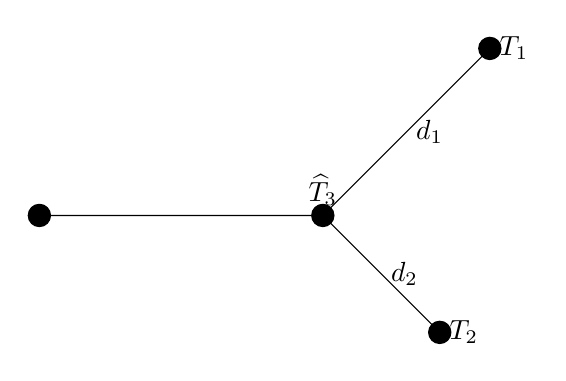
\begin{tikzpicture}[scale=3]
			\coordinate (node) at (0, 0);
			\coordinate (child1) at (45:1);
			\coordinate (child2) at (-45:.7);
			\coordinate (parent) at (180:1.2);
			\draw node at (node) [shape=circle, draw, fill=black, inner sep=.1cm] {}
				node at (child1) [shape=circle, draw, fill=black, inner sep=.1cm] {}
				node at (child2) [shape=circle, draw, fill=black, inner sep=.1cm] {}
				node at (parent) [shape=circle, draw, fill=black, inner sep=.1cm] {};
			\draw (node) -- node [anchor=west] {$d_1$} (child1) node [anchor=west] {$T_1$} (node) -- node [anchor=west] {$d_2$} (child2) node [anchor=west] {$T_2$} (node) -- (parent);
			\draw (node) node [anchor=south] {$\widehat{T}_3$};
		\end{tikzpicture}
		\caption{In the initial seeding step each internal node is assigned times based on a local maximum likelihood. Here node 3 is estimated by $\widehat{T}_3$ from the times of its child node ($T_1$ and $T_2$) and the genetic distance of the edges between them ($d_1$ and $d_2$).}
		\label{fig:nodedatingprior}
	\end{subfigure}
	\begin{subfigure}[ht]{8cm}
		\centering
		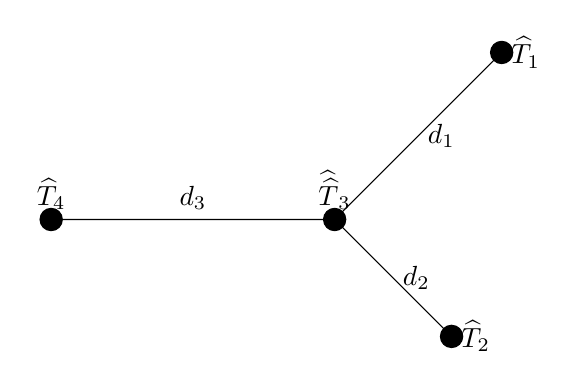
\begin{tikzpicture}[scale=3]
			\coordinate (node) at (0, 0);
			\coordinate (child1) at (45:1);
			\coordinate (child2) at (-45:.7);
			\coordinate (parent) at (180:1.2);
			\draw node at (node) [shape=circle, draw, fill=black, inner sep=.1cm] {}
				node at (child1) [shape=circle, draw, fill=black, inner sep=.1cm] {}
				node at (child2) [shape=circle, draw, fill=black, inner sep=.1cm] {}
				node at (parent) [shape=circle, draw, fill=black, inner sep=.1cm] {};
			\draw (node) -- node [anchor=west] {$d_1$} (child1) node [anchor=west] {$\widehat{T}_1$} (node) -- node [anchor=west] {$d_2$} (child2) node [anchor=west] {$\widehat{T}_2$} (node) -- node [anchor=south] {$d_3$} (parent) node [anchor=south] {$\widehat{T}_4$};
			\draw (node) node [anchor=south] {$\widehat{\widehat{T}}_3$};
		\end{tikzpicture}
		\caption{Then using these estimates, the algorithm iterates including the parent's time ($\widehat{T}_4$) and the genetic distance of the edge between the node and the parent ($d_3$) and also the updated times of the children nodes.}
		\label{fig:nodedatingiter}
	\end{subfigure}
	\caption[Local node dating]{Local node dating methodology}
	\label{fig:nodedating}
\end{figure}
%\end{comment}

%%%%%%%%%%%%%%%  TABLES  %%%%%%%%%%%%%%%

\end{document}
